%% Use the "normalphoto" option if you want a normal photo instead of cropped to a circle
% \documentclass[10pt,a4paper,normalphoto]{altacv}

\documentclass[10pt,a4paper,ragged2e,withhyper]{altacv}
%% AltaCV uses the fontawesome5 and simpleicons packages.
%% See http://texdoc.net/pkg/fontawesome5 and http://texdoc.net/pkg/simpleicons for full list of symbols.

% Change the page layout if you need to
\geometry{left=1.25cm,right=1.25cm,top=1.5cm,bottom=1.5cm,columnsep=1.2cm}

% The paracol package lets you typeset columns of text in parallel
\usepackage{paracol}


% Change the font if you want to, depending on whether
% you're using pdflatex or xelatex/lualatex
% WHEN COMPILING WITH XELATEX PLEASE USE
% xelatex -shell-escape -output-driver="xdvipdfmx -z 0" mmayer.tex
\iftutex
  % If using xelatex or lualatex:
  \setmainfont{Lato}
\else
  % If using pdflatex:
  \usepackage[default]{lato}
\fi

% Change the colours if you want to
\definecolor{AlmostBlack}{HTML}{0D0D0D}
\definecolor{VividPurple}{HTML}{3E0097}
\definecolor{SlateGrey}{HTML}{2E2E2E}
\definecolor{LightGrey}{HTML}{666666}
% \colorlet{name}{black}
\colorlet{tagline}{SlateGrey}
\colorlet{heading}{AlmostBlack}
\colorlet{headingrule}{AlmostBlack}
% \colorlet{subheading}{PastelRed}
\colorlet{accent}{AlmostBlack}
\colorlet{emphasis}{SlateGrey}
\colorlet{body}{LightGrey}



\renewcommand{\cvItemMarker}{{\small\textbullet}}
\renewcommand{\cvRatingMarker}{\faCircle}
\renewcommand{\taglinefont}{\LARGE\bfseries}
\usepackage{tikz}
\newcommand{\maindivider}{%
  \noindent
  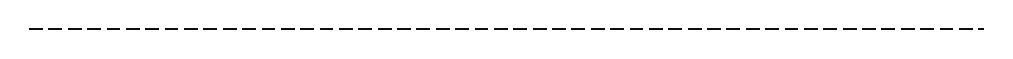
\begin{tikzpicture}
    \draw[headingrule, line width=1pt, dash pattern=on 5pt off 2pt] (0,0) -- (\linewidth,0);
  \end{tikzpicture}\par\vspace{0.3em}%
}
\input{pubs-num.tex}

%% sample.bib contains your publications
\addbibresource{sample.bib}

\begin{document}
\name{Adrien Sourdille}
\tagline{Ingénieur Analytics}
% Cropped to square from https://en.wikipedia.org/wiki/Marissa_Mayer#/media/File:Marissa_Mayer_May_2014_(cropped).jpg, CC-BY 2.0
% \photoL{2cm}{images/Yacht_High,images/Suitcase_High}
\personalinfo{%
  \email{adriensourdille99@gmail.com}
  \phone{+33 (0)7 85 76 66 85}
  \location{Paris, France}
  \linkedin{adrien-sourdille}
  \github{AdrienSourdilleTIL}
}

\makecvheader

%% Depending on your tastes, you may want to make fonts of itemize environments slightly smaller
\AtBeginEnvironment{itemize}{\small}

%% Set the left/right column width ratio to 6:4.
\columnratio{0.6}

% Start a 2-column paracol. Both the left and right columns will automatically
% break across pages if things get too long.
\begin{paracol}{2}

\cvsection{Expérience Professionnelle}

\cvevent{Consultant Data Analyst \& Data Engineer}{The Information Lab}{Février 2023 -- En cours}{Londres, Royaume-Uni}
\begin{itemize}
\item Formation intensive de 4 mois au sein d’un cabinet de conseil data, suivie de 3 ans de missions en Data Engineering et Analytics : conception de pipelines ETL, automatisation de rapports, création de dashboards interactifs et mise en place de systèmes prédictifs pour optimiser l’allocation des ressources. Compétences avancées en Snowflake, GCP, Azure, dbt, Tableau et Alteryx, avec un focus sur la transformation de données complexes en informations exploitables.
\end{itemize}

\maindivider

\cvevent{Data Engineer}{Consultant en mission chez Virgin Media O2}{Août 2025 -- En cours}{Londres, Royaume-Uni}

\begin{itemize}
\item Conception et développement d’un pipeline innovant reliant les données de performance réseau aux métriques clients, permettant de mesurer de bout en bout l’impact d’un investissement de 700M~\textsterling{} sur les performances réseau, la satisfaction, le churn et les revenus.
\item Mise en place d’un système pour identifier les moments critiques dans le parcours utilisateur et prioriser les améliorations d’infrastructure à forte valeur ajoutée.
\end{itemize}
\vspace{0.1cm}
\cvtag{GCP}
\cvtag{SQL}
\cvtag{dbt}
\cvtag{Jira}
\cvtag{Gitlab}

\divider

\cvevent{Data Engineer}{Consultant en mission chez Prêt a Manger}{Novembre 2024 -- Juin 2025}{Londres, Royaume-Uni}
\begin{itemize}
\item Création du pipeline ETL centrale pour la migration SQL Server → Snowflake, permettant des économies de plusieurs millions d’euros sur l’infrastructure et les licences.
\item Transformation des données transactionnelles de 431 magasins en informations exploitables sur le CA, stocks, taxes et pertes, et réduction du temps de reporting de 92\% par rapport au processus manuel.
\item Refonte et amélioration d’un outil stratégique exploitant les flux de transactions pour anticiper les besoins en personnel et optimiser la gestion des caissiers en temps réel.
\end{itemize}
\vspace{0.1cm}
\cvtag{Snowflake}
\cvtag{SQL}
\cvtag{Github}
\cvtag{Javascript}
\cvtag{Jira}
\cvtag{GCP}
\cvtag{Azure}

\divider

\cvevent{Data Analyst}{Consultant en mission chez BAE Systems}{Juin 2023 -- Juin 2024}{Londres, Royaume-Uni}
\begin{itemize}
\item Cadrage, développement et automatisation d’un reporting financier permettant le suivi du budget et des dépenses R\&D d’un portefeuille de plusieurs centaines de millions d’euros, améliorant la fiabilité et la disponibilité des données financières. 
\item Conception et déploiement de dashboards pour le suivi des investissements technologiques, améliorant la compréhension des données dans la chaîne de décision et multipliant leur utilisation mensuelle par 4.
\end{itemize}
\vspace{0.1cm}
\cvtag{Tableau Suite}
\cvtag{Alteryx Suite}
\cvtag{Jira}

\switchcolumn

\cvsection{Formation}

\cvevent{Master en Science des Données Géographiques}{London School of Economics (LSE)}{2021 -- 2022}{Londres, Royaume-Uni}

Formation en data science appliquée :
apprentissage par renforcement, visualisations Python, SIG et analyse spatiale. Méthodes économétriques et recherche causale, avec un accent sur l’économie environnementale. Thèse sur l’impact des certificats énergétiques (DPE) sur les prix de l’immobilier en France, utilisant des méthodes rigoureuses pour extraire des insights fiables.


\cvsection{Profil}


{\color{SlateGrey} \itshape \normalsize
Ingénieur Analytics avec 3 ans d’expérience en conseil, spécialisé dans la transformation de données complexes en décisions opérationnelles à fort impact. Expérimenté dans la conception de pipelines ETL, la mise en place de rapports automatisés et la création de dashboards interactifs, avec une expertise avancée en Snowflake, dbt, Tableau et Alteryx. Passionné par l’utilisation des données pour éclairer les décisions et rendre l’information accessible à tous, afin de soutenir des solutions collectives et rationnelles pour la transition énergétique.
}

\cvsection{Certifications}

\begin{minipage}[c]{0.08\linewidth}
  
\includegraphics[width=\linewidth]{images/tableau-certified-data-analyst.png}
\end{minipage}%
\hspace{0.5em}%
\begin{minipage}[c]{0.9\linewidth}
  \textbf{Tableau Data Analyst}
\end{minipage}

\vspace{0.5em}

\begin{minipage}[c]{0.08\linewidth}
  
\includegraphics[width=\linewidth]{images/Snowpro-core.png}
\end{minipage}%
\hspace{0.5em}%
\begin{minipage}[c]{0.9\linewidth}
  \textbf{SnowPro Core}
\end{minipage}

\vspace{0.5em}

\begin{minipage}[c]{0.08\linewidth}
  
\includegraphics[width=\linewidth]{images/alteryx-designer-advanced-certification.png}
\end{minipage}%
\hspace{0.5em}%
\begin{minipage}[c]{0.9\linewidth}
  \textbf{Alteryx Designer Advanced}
\end{minipage}


\cvsection{Stack}

% Don't overuse these \cvtag boxes — they're just eye-candies and not essential. If something doesn't fit on a single line, it probably works better as part of an itemized list (probably inlined itemized list), or just as a comma-separated list of strengths.

% The `ragged2e` document class option might cause automatic linebreaks between \cvtag to fail.
% Either remove the ragged2e option; or
% add \LaTeXraggedright in the paragraph for these \cvtag
\cvtag{Tableau Suite}
\cvtag{Alteryx Suite}
\cvtag{SQL}
\cvtag{dbt}
\cvtag{Javascript}
\cvtag{Python}
\cvtag{Jira}
\cvtag{Github}
\cvtag{Gitlab}
\cvtag{Snowflake}
\cvtag{GCP}
\cvtag{Azure}

\cvsection{Langues}

\cvskill{Anglais}{5}
% \divider

\cvskill{Français}{5}
% \divider

\cvskill{Italien}{3.5} %% supports X.5 values.

\vspace{0.5cm}

\href{https://adriensourdilletil.github.io/AdrienSourdillePortfolio/}{\faBriefcase\ Visiter mon Portfolio}

\vspace{0.25cm}

\href{https://public.tableau.com/app/profile/adrien.sourdille4093/vizzes}{\faHome\ Visiter mon Tableau Public}


\end{paracol}

\end{document}
